\documentclass{article}
\usepackage{amsmath}
\usepackage{graphicx}

\begin{document}

\section{Fragile Watermark Preparation}

The host image is divided into $2 \times 4$ size non-overlapping blocks (total blocks $= \text{TB}$). A random binary sequence $W_{ran\_2}$ is produced using $K_3$ (secret key-3) with the help of SFMT generator of length $6 \times \text{TB}$. The average block intensities of every $2 \times 4$ are converted into 8-bit binary representation. The 6 MSB (most significant bits) of these 8 bits are concatenated in a controlled randomized manner using $K_4$ (secret key-4) to generate recovery watermark data ($W_{recov}$). Now, every 6 bits from both sequences (i.e., $W_{ran\_2}$ and $W_{recov}$) are cascaded. Finally, the combined watermark $W_{fragile+recov}$ is obtained from this cascading. Figure \ref{fig:preparation} presents the process of generating the watermark $W_{fragile+recov}$.

\begin{figure}[h]
    \centering
    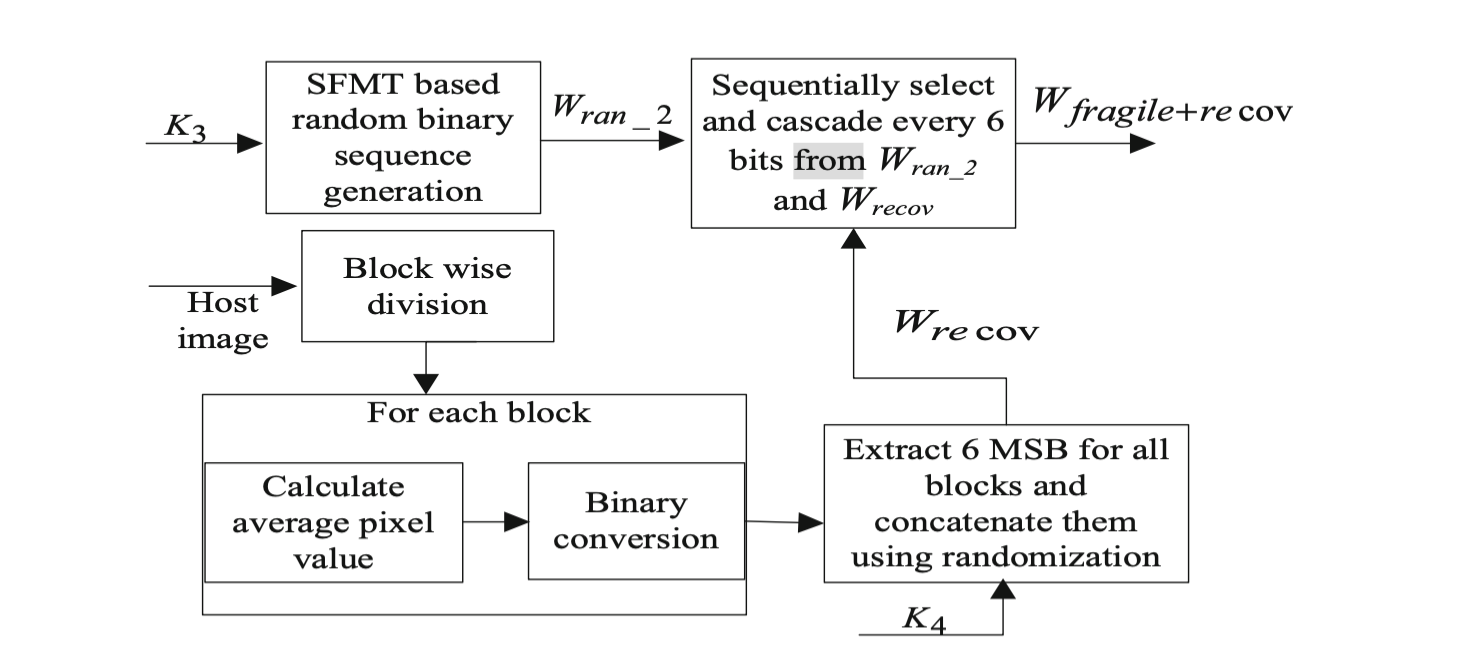
\includegraphics[width=0.8\textwidth]{watermark_preparation_process.png}
    \caption{Fragile watermark preparation in order to preserve the recovery data along with the authentication data}
    \label{fig:preparation}
\end{figure}

\section{Fragile Embedding}

The following steps show the embedding of the watermark ($W_{\text{fragile+recov}}$) into the image (Watermarked\textsubscript{r}).

\begin{itemize}
    \item \textbf{Step-1} Divide the image (Watermarked\textsubscript{r}) into $2 \times 4$ size of non-overlapping blocks. Then, sequentially select 12 bits of watermark data from $W_{\text{fragile+recov}}$ for each block.
    
    \item \textbf{Step-2} Choose the first block and consider that each column is representing a pixel unit (with 2 pixels). Thus, each $2 \times 4$ size block has four units (e.g., U1, U2, U3, and U4).
    
    \item \textbf{Step-3} Convert 12-bit watermark into 9-base number $Wat_9$ in such a way that it has four digits (e.g., $Wat_9 = d1d2d3d4$).
    
    \item \textbf{Step-4} Modify pixels of U1 using $d1$ as per the given steps.
    \begin{itemize}
        \item Compute digit $F_{\text{embed}}$ as shown in Eq. (5). Here, $P_k$ is the $k^{\text{th}}$ pixel of unit U.
        \[
        F_{\text{embed}} = \left( \sum_{k=1}^n 3^{k-1} P_k \right) \mod 3^n \quad \text{where} \quad n = 2
        \]
        
        \item Calculate $x$ as given in Eq. (6).
        \[
        x = \left( d - F_{\text{embed}} + \left\lfloor \frac{3^n - 1}{2} \right\rfloor \right) \mod 3^n
        \]
        
        \item Change $x$ into $x'$ by converting into 3-base number as $x' = y_1 y_2 \ldots y_n$, where $y_i$ denotes the $i^{\text{th}}$ digit of $x'$ for $1 \leq i \leq n$. Next, get $x'' = z_1 z_2 \ldots z_n$, where $z_i = y_i - 1$.
        
        \item Add digits of $x''$ to the pixels of unit U to get the updated pixels as shown in Eq. (7).
        \[
        P_{\text{new}_k} = P_k + z_i \quad \text{where} \quad
        \begin{cases}
            1 \leq k \leq n \\
            i = n - k + 1
        \end{cases}
        \]
    \end{itemize}
    
    \item Repeat the steps with U2, U3, and U4 to embed $d2$, $d3$, and $d4$, respectively.
    
    \item \textbf{Step-5} Repeat step 2, 3, and 4 for each block to get the dual watermarked image $W_{\text{img}}$.
\end{itemize}

\section{Fragile Watermark Extraction (Tamper Check)}

The following steps show the authentication process to check the tampering:

\begin{enumerate}
    \item Divide the attacked watermarked image into $2 \times 4$ size blocks and extract the four digits ($F_{ext}$) using Eq. (5) from each block.
    
    \item Convert the four-digit 9-base number (i.e., $F_{ext\_1}F_{ext\_2}F_{ext\_3}F_{ext\_4}$) into binary (i.e., 12-bit size). Similarly, extract 12-bit numbers from each block.
    
    \item Get $EW_{ran\_2}$ by concatenating initial 6-bits concerning each block. Likewise, get $EW_{recov}$ by cascading the last 6 bits related to each block.
    
    \item Generate binary sequence $W_{ran\_2}$ using $K_3$-based SFMT process and Eq. (1). Further, compare the corresponding bits of $EW_{ran\_2}$ and $W_{ran\_2}$ to authenticate the image. If the bits are different, then the concerning block is marked as tampered.
    
    \item Apply the block-neighborhood approach to smoothen the result of Step 4. For smoothing, eight neighborhood blocks (except corner positions) of each block are considered. If the majority of the blocks (out of these nine blocks) are tampered/non-tampered, the block is also marked as tampered/non-tampered.
\end{enumerate}

\end{document}
